% vi:ft=tex
\documentclass{standalone}

\usepackage{tikz}
\usepackage{verbatim}
\usepackage{mathtools}

\usetikzlibrary{arrows}
\usetikzlibrary{calc}

\begin{document}

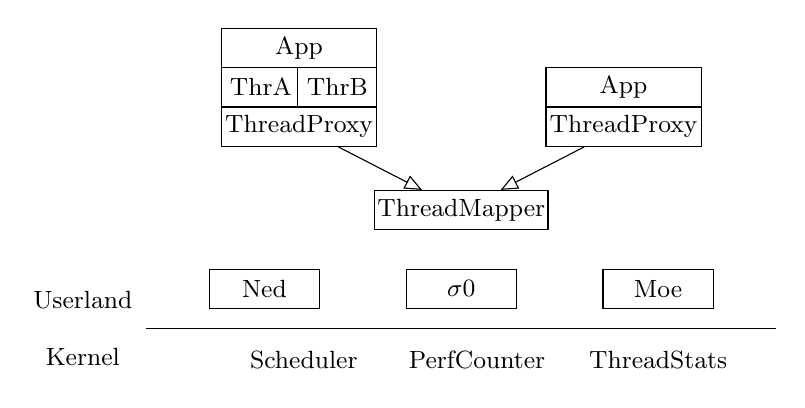
\begin{tikzpicture}[node distance=1.5cm]

  % Colors
  % Styles
  \tikzstyle{defaultRec} = [font=\small, text centered, inner sep = 1pt,
    draw=none, shape=rectangle, fill=white, minimum height = .5cm, minimum
  width = 1.4cm];
  \tikzstyle{tpRec} = [defaultRec, draw=black,text width=1.9cm];
  \tikzstyle{threadRec} = [defaultRec, draw=black, node distance=0mm,
  minimum width=1cm]
  \tikzstyle{arrow} = [-open triangle 45, black];

  % Variables

  % Drawing

  \draw[black, thin] (0,0) -- (8,0);
  \node[defaultRec, anchor=south east] at (-1mm,1mm) {Userland};
  \node(tm) [defaultRec, draw] at (4cm, 1.5cm) {ThreadMapper};
  \node [defaultRec, draw] at (1.5cm,.5cm) {Ned};
  \node [defaultRec, draw] at (4cm, .5cm) {$\sigma{}0$};
  \node [defaultRec, draw] at (6.5cm,.5cm) {Moe};
  \node[defaultRec, anchor=north east] at (-1mm,-1mm) {Kernel};
  \node[defaultRec] at (2cm, -4mm) {Scheduler};
  \node[defaultRec] at (4.2cm, -4mm) {PerfCounter};
  \node[defaultRec] at (6.5cm, -4mm) {ThreadStats};

      \node(tp1) [tpRec, above left of=tm,xshift=-1cm] {ThreadProxy};
      \draw[transparent] (tp1.west) -- +(0,5mm) coordinate(helpWest);
      \node(t1.1) [threadRec, right of=helpWest,anchor=west,] {ThrA};

      \draw[transparent] (tp1.east) -- +(0,5mm) coordinate(helpEast);
      \node(t1.2) [threadRec, right of=helpEast,anchor=east,] {ThrB};

      \node(a1)	[tpRec, above of=tp1, node distance=1cm] {App};

      \node(tp2) [tpRec, above right of=tm,xshift=1cm] {ThreadProxy};
      \node(a2)	[tpRec, above of=tp2, node distance=5mm] {App};

      \draw [arrow] (tp1) to (tm);
      \draw [arrow] (tp2) to (tm);

\end{tikzpicture}

\end{document}
